%% EXOPLANETS 6 poster: Photoevaporation traced by Lya, Ha, He I 10830
%% A1 portrait, 90% (53.5 x 75.7 cm).  Build: pdflatex WASP-52b_poster.tex
\documentclass[final]{beamer}
\usepackage[orientation=portrait,size=custom,width=53.5,height=75.7,scale=0.85]{beamerposter}
\usepackage{graphicx}
\usepackage{booktabs}
\usepackage{amsmath,amssymb}
\usepackage{tcolorbox}
\graphicspath{{figs/}}

%% Times-family fonts (text + math)
\usefonttheme{professionalfonts}
\usepackage{newtxtext,newtxmath}

%% looser line spacing + a little air between list items
\linespread{1.18}
\setlength{\parskip}{4pt}
\setbeamertemplate{itemize/enumerate body begin}{\setlength{\itemsep}{6pt}}

%% ---- colors & block style ----
\definecolor{kasiblue}{RGB}{20,58,107}
\definecolor{kasilight}{RGB}{232,238,247}
\definecolor{accent}{RGB}{196,90,17}
\setbeamercolor{block title}{fg=white,bg=kasiblue}
\setbeamercolor{block body}{fg=black,bg=kasilight}
\setbeamercolor{block alerted title}{fg=white,bg=accent}
\setbeamercolor{block alerted body}{fg=black,bg=accent!12}
\setbeamerfont{block title}{size=\large,series=\bfseries}
\setbeamertemplate{navigation symbols}{}
\setbeamertemplate{caption}{\insertcaption}
\setbeamertemplate{itemize items}{\textbullet}

%% equal-height columns: fixed column body height, \vfill distributes the slack
\newlength{\colht}\setlength{\colht}{0.848\paperheight}

\newcommand{\Rp}{R_{\rm p}}
\newcommand{\Fo}{F_{0}}
\newcommand{\Mdot}{\dot{M}}

\begin{document}
\begin{frame}[t]{}

%% ================= TITLE HEADER =================
\begin{tcolorbox}[colback=kasiblue,colframe=kasiblue,sharp corners,boxrule=0pt,
  left=12mm,right=12mm,top=6mm,bottom=6mm]
\begin{center}
{\color{white}\Huge\bfseries Photoevaporation in Hot Jupiter Atmospheres\par}
\vspace{3mm}
{\color{white}\Large\bfseries Traced by Ly$\alpha$, H$\alpha$, and He\,I\,$\lambda$10830 Triplet Lines\par}
\vspace{6mm}
{\color{white}\large Kwang-Il Seon$^{1,2}$ \quad\&\quad Jisan Yu$^{1,2}$\par}
\vspace{2mm}
{\color{kasilight}\normalsize $^{1}$Korea Astronomy \& Space Science Institute \quad
$^{2}$Department of Astronomy \& Space Science, University of Science and Technology\par}
\vspace{2mm}
{\color{kasilight}\normalsize EXOPLANETS\,6 \,\textbullet\, 29 June -- 03 July 2026 \,\textbullet\, Porto, Portugal\par}
\end{center}
\end{tcolorbox}
\vspace{6mm}

\begin{columns}[t]

%% ================= LEFT COLUMN =================
\begin{column}{0.475\paperwidth}
\begin{minipage}[t][\colht][s]{\linewidth}

\begin{block}{1. Motivation: three lines, three layers}
\begin{itemize}
\item Close-in giants lose mass through \textbf{XUV-driven hydrodynamic escape}
  (photoevaporation). Resonance/metastable lines probe the escaping gas at
  \emph{complementary} layers:
  \begin{itemize}
  \item \textbf{Ly$\alpha$} (H\,$1s$): bulk neutral H (resonant; core lost to ISM).
  \item \textbf{H$\alpha$} (H\,$n{=}2$): Ly$\alpha$-pumped excited H; optical.
  \item \textbf{He\,I\,$\lambda$10830} (He\,$2^3S$ metastable): near-IR.
  \end{itemize}
\item Modeling the lines \emph{jointly} constrains the H/He composition, the
  mass-loss rate, and the (usually unobserved) stellar Ly$\alpha$ flux.
\item We model the inflated hot Jupiter \textbf{WASP-52b} (K2V host) with the
  \textbf{EXHALE} escape code coupled to the \textbf{LaRT} Ly$\alpha$ Monte-Carlo code.
\end{itemize}
\end{block}

\vfill

\begin{block}{2. Line formation: He\,$2^3S$ \& H$\alpha$ Ly$\alpha$-pumping}
\centering
\begin{minipage}[c]{0.47\linewidth}\centering
  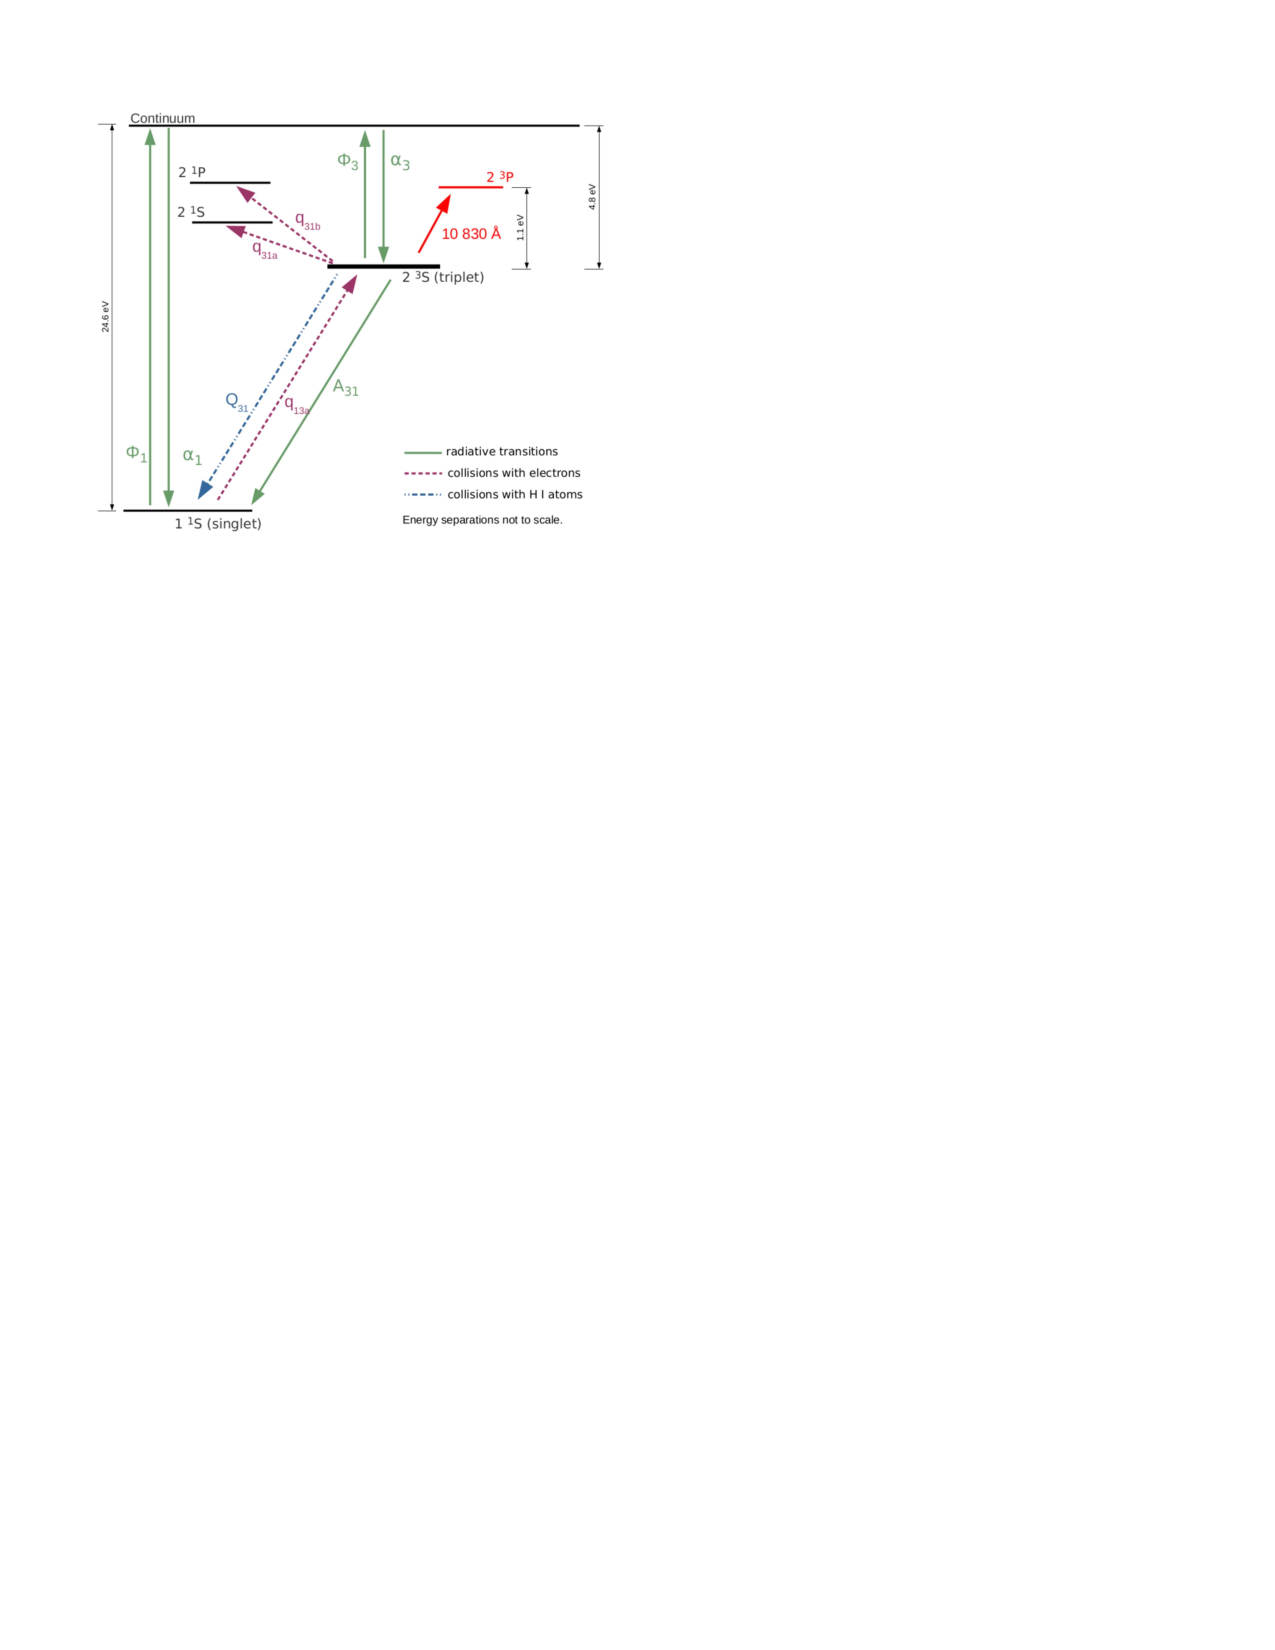
\includegraphics[width=\linewidth]{fig_He10833.pdf}
\end{minipage}\hfill
\begin{minipage}[c]{0.42\linewidth}\centering
  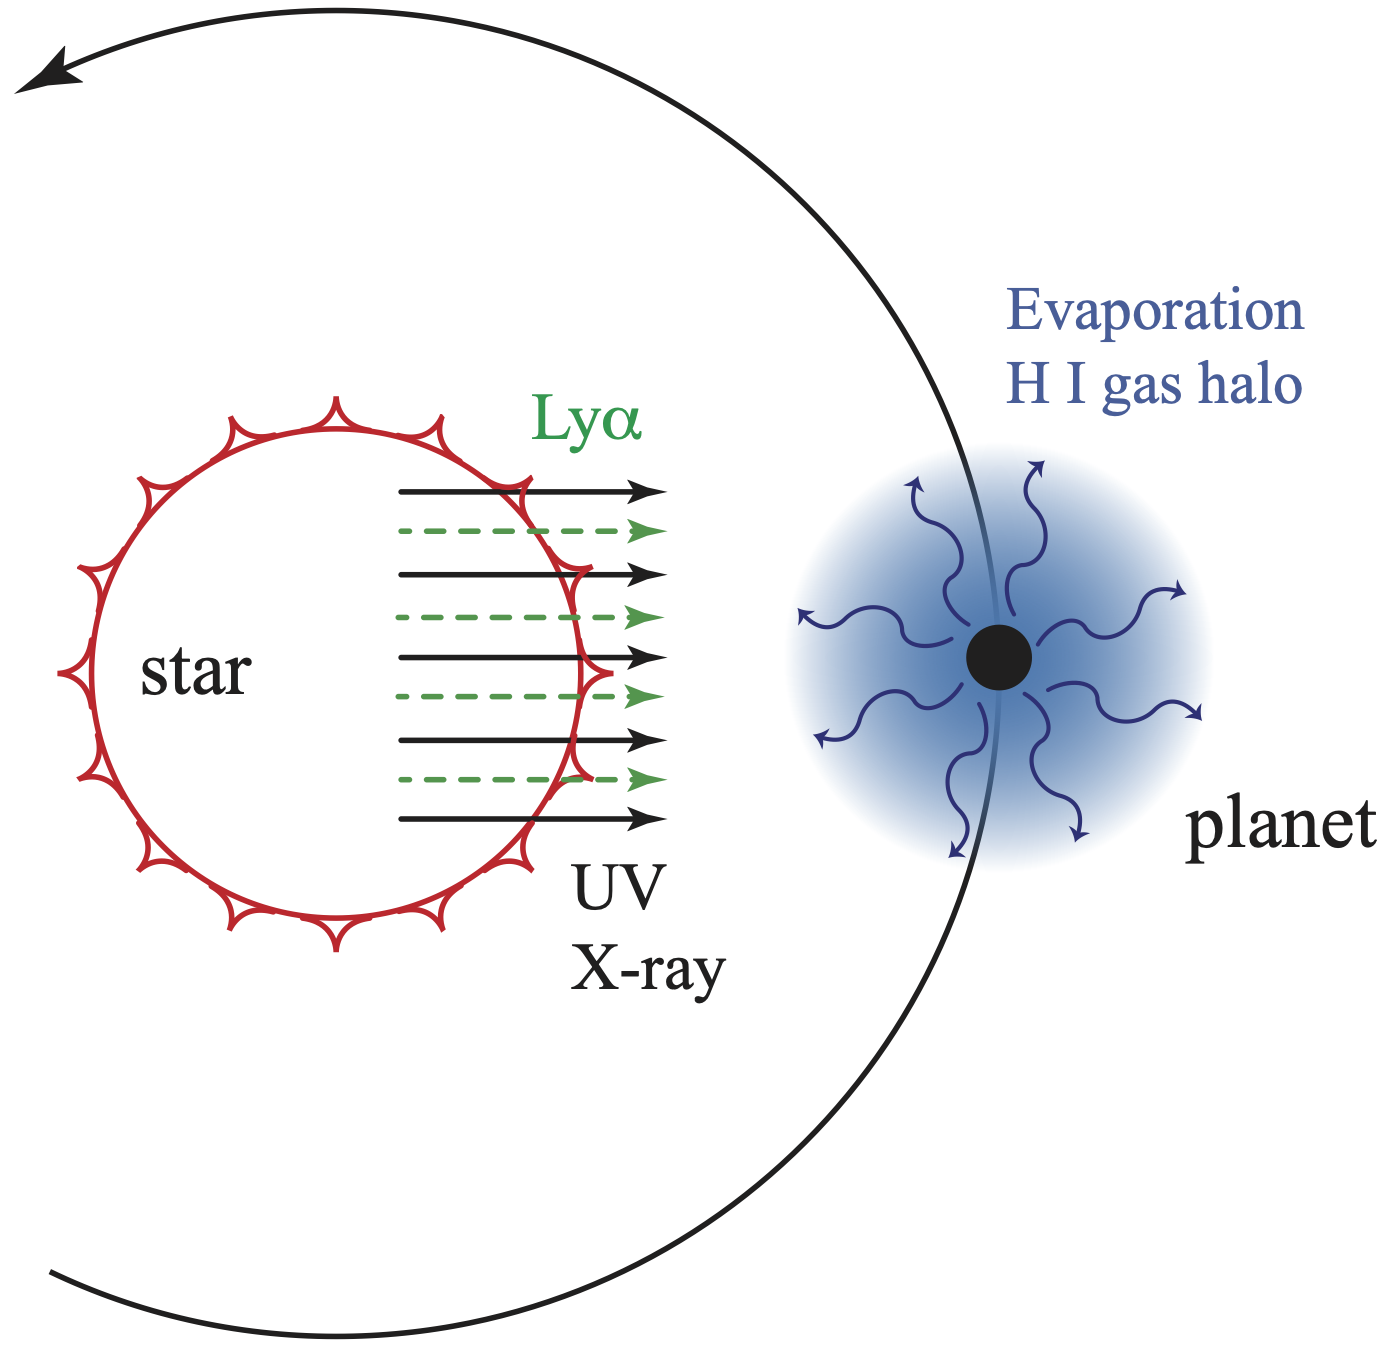
\includegraphics[width=0.56\linewidth]{fig_Ha_a.png}\\[2mm]
  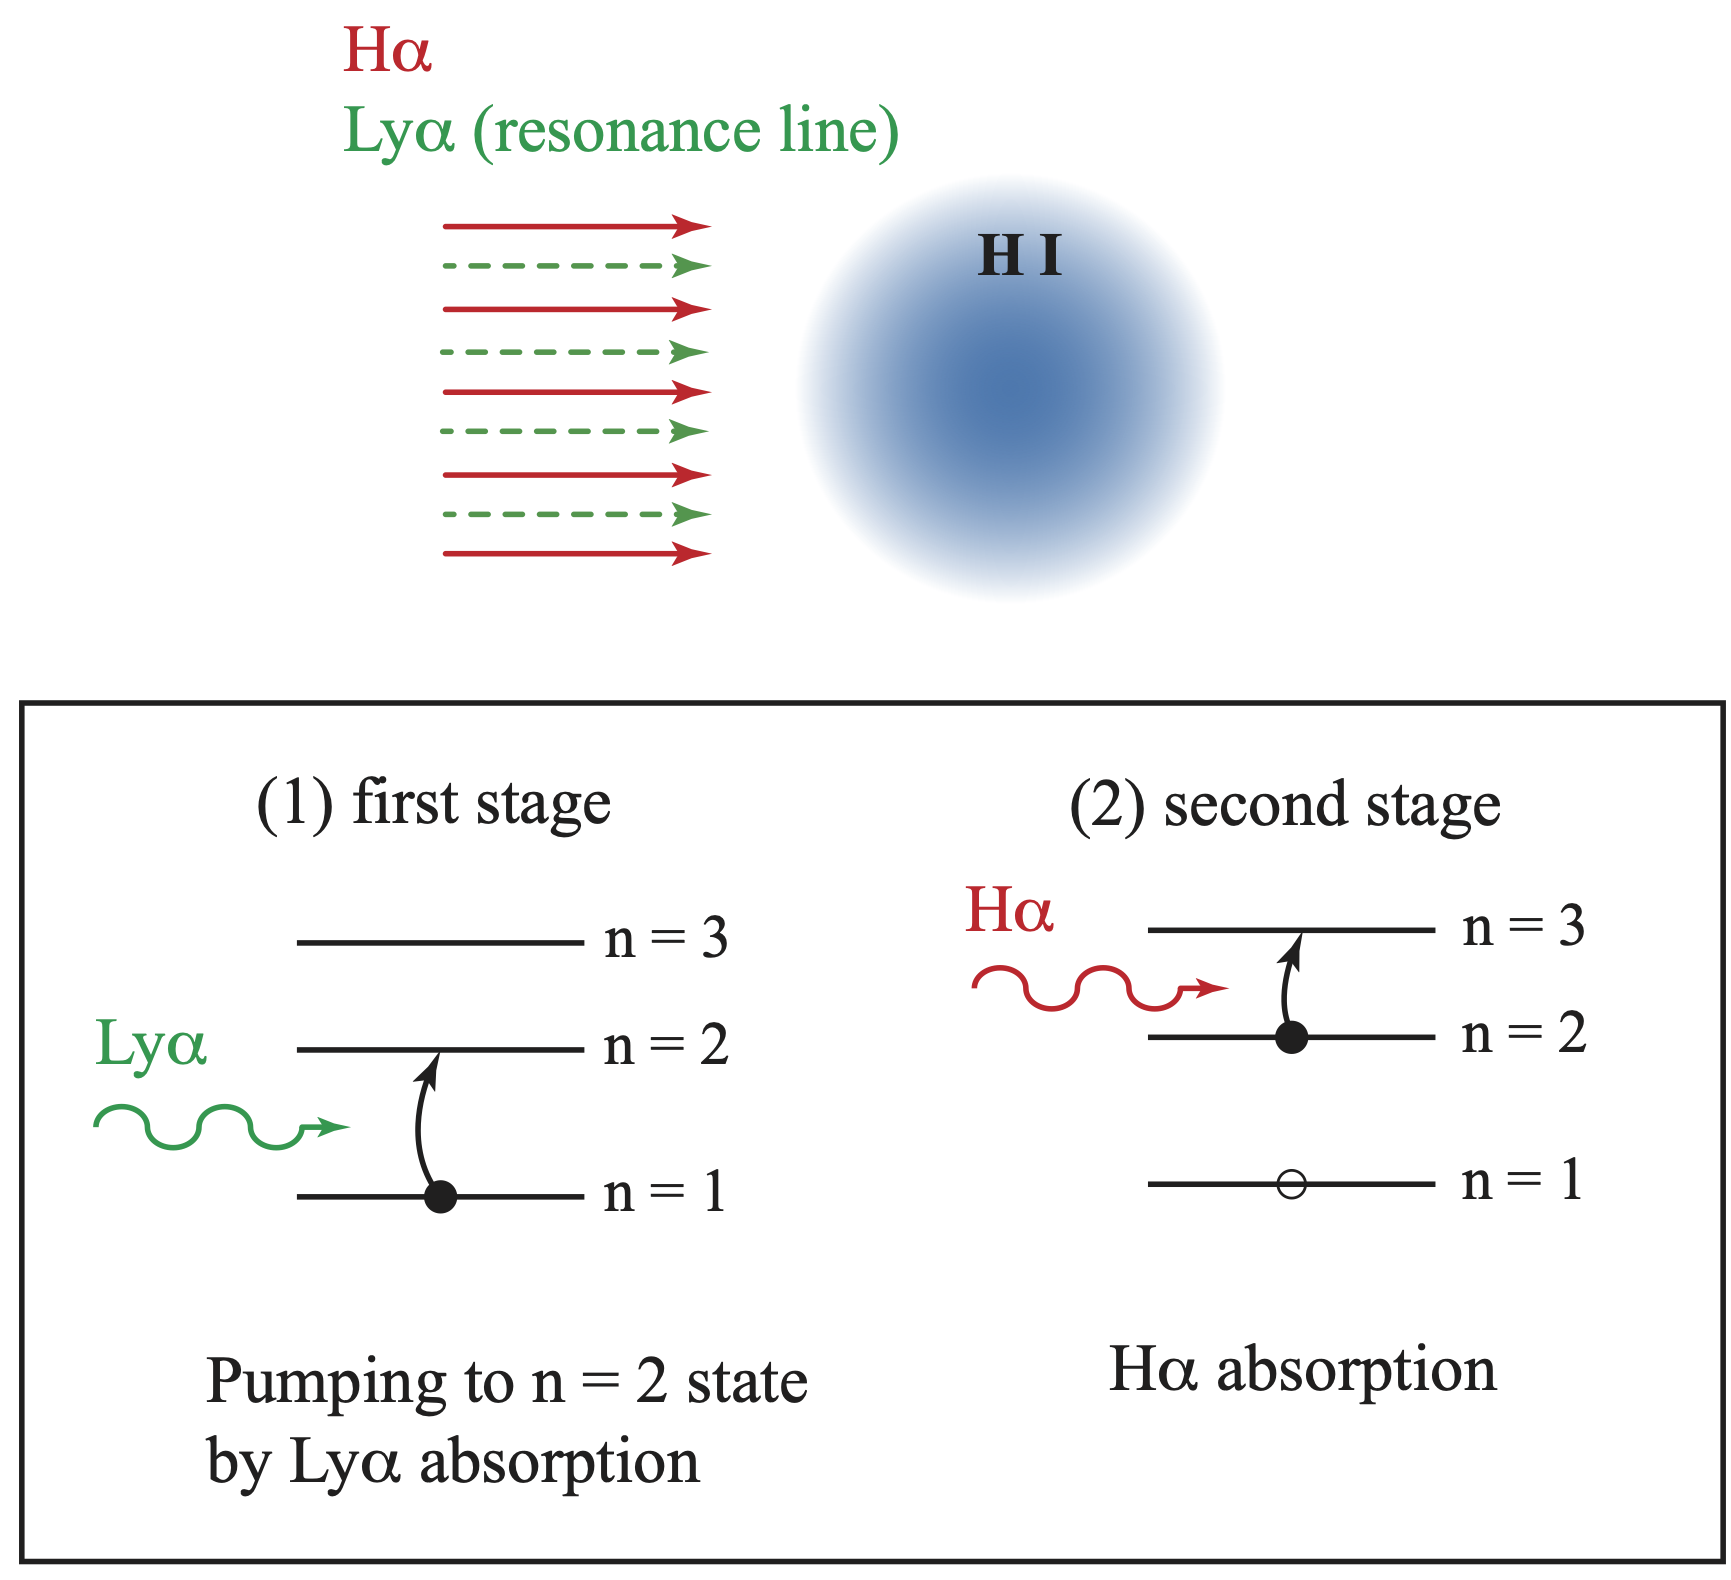
\includegraphics[width=0.56\linewidth]{fig_Ha_b.png}
\end{minipage}\\[1mm]
\raggedright\footnotesize
\textbf{He\,10830} (left): metastable He\,$2^3S$ ($2^3S\!\to\!2^3P$), fed by
recombination$+$cascade, drained by FUV photoionization.
\textbf{H$\alpha$} (right; $n{=}2\!\to\!3$) needs an enhanced $n{=}2$ set mainly by
\textbf{Ly$\alpha$ pumping} of $1s\!\to\!2p$.
\end{block}

\vfill

\begin{block}{3. EXHALE: code \& algorithms}
\begin{itemize}
\item \textbf{1-D multi-species radiation-hydrodynamics} (extended ATES,
  Caldiroli+2021): mass/momentum/energy Euler equations $\to$ steady state, with
  the full \textbf{Roche} potential (tidal $+$ centrifugal; $L_1$-truncated or extended).
\item \textbf{Ionization equilibrium} of H, He $+$ metals (C,N,O,Mg,Si,Ca,Na,K,S,Fe)
  via Newton/MINPACK; photoionization, collisional ionization,
  (Badnell) radiative$+$dielectronic recombination, charge exchange.
\item \textbf{Heating} XUV photoionization; \textbf{cooling} closed-form CHIANTI
  metal lines $+$ Ly$\alpha$ $+$ recombination $+$ bremsstrahlung.
\item \textbf{He\,$2^3S$} metastable network $\to$ He\,10830; \textbf{H\,$n{=}2$}
  $\to$ H$\alpha$ (Christie+2013 NLTE $+$ Ly$\alpha$ pumping).
\item \textbf{Steady solver:} PLM$\to$WENO3 march $+$ Newton/JFNK (flux convergence);
  \textbf{transmission} via Voigt LOS $+$ disk average (\texttt{EXHALE\_transit.py}).
\item \textbf{Ly$\alpha$ RT:} coupled to \textbf{LaRT} 3-D Monte Carlo (Seon \& Kim
  2020) $\to$ cylindrical $P_\alpha(\rho,z)$ $\to$ 2-D $n_{2p}$ $\to$ H$\alpha$.
\end{itemize}
\end{block}

\vfill

\begin{block}{4. WASP-52b model setup}
\begin{itemize}
\item Planet/star (Yan+2022): $M_\star=0.87\,M_\odot$, $R_\star=0.79\,R_\odot$ (K2V);
  $M_{\rm p}=0.46\,M_{\rm J}$, $\Rp=1.27\,R_{\rm J}$, $T_{\rm eq}=1304$\,K,
  $a=0.0272$\,au.
\item Stellar SED: $\epsilon$\,Eri (MUSCLES) scaled to the orbit;
  $F_{\rm XUV}=3.4\times10^{4}\,\mathrm{erg\,cm^{-2}\,s^{-1}}$, hardness
  $\beta_m\equiv F(1\text{--}100\,\text{\AA})/F(1\text{--}912\,\text{\AA})=0.218$.
\item Lower boundary pressure-anchored at $1\,\mu$bar; full Roche potential
  ($L_1$ at $\sim\!2.53\,\Rp$). Converged wind: $T$ peaks $\sim\!10^4$\,K near
  $2\,\Rp$, transonic, density falling $\sim$7 dex over $1$--$2.5\,\Rp$.
\item \textbf{Validation:} the steady-state mass-loss rate reproduces Yan+2022
  (Table 4) to within $\sim$10\% at every XUV flux.
\end{itemize}
\centering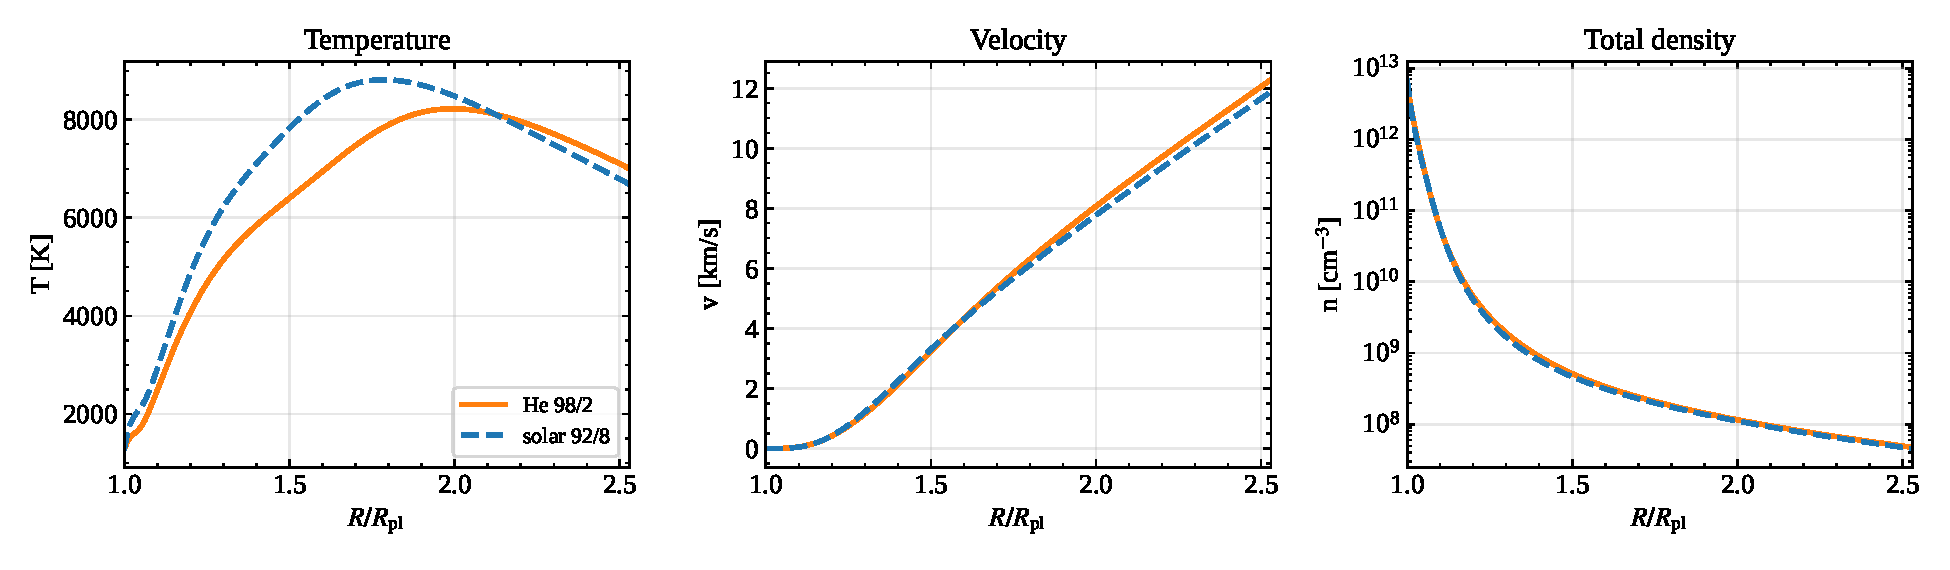
\includegraphics[width=0.80\linewidth]{profiles.pdf}\\[0.5mm]
{\footnotesize Best-fit wind ($\mathbf{H/He\,98/2}$, $L_1$ domain; solar shown for reference).}
\end{block}

\end{minipage}
\end{column}

%% ================= RIGHT COLUMN =================
\begin{column}{0.475\paperwidth}
\begin{minipage}[t][\colht][s]{\linewidth}

\begin{block}{5. He\,I\,$\lambda$10830: domain \& composition}
\begin{columns}[T]
\begin{column}{0.5\linewidth}\centering
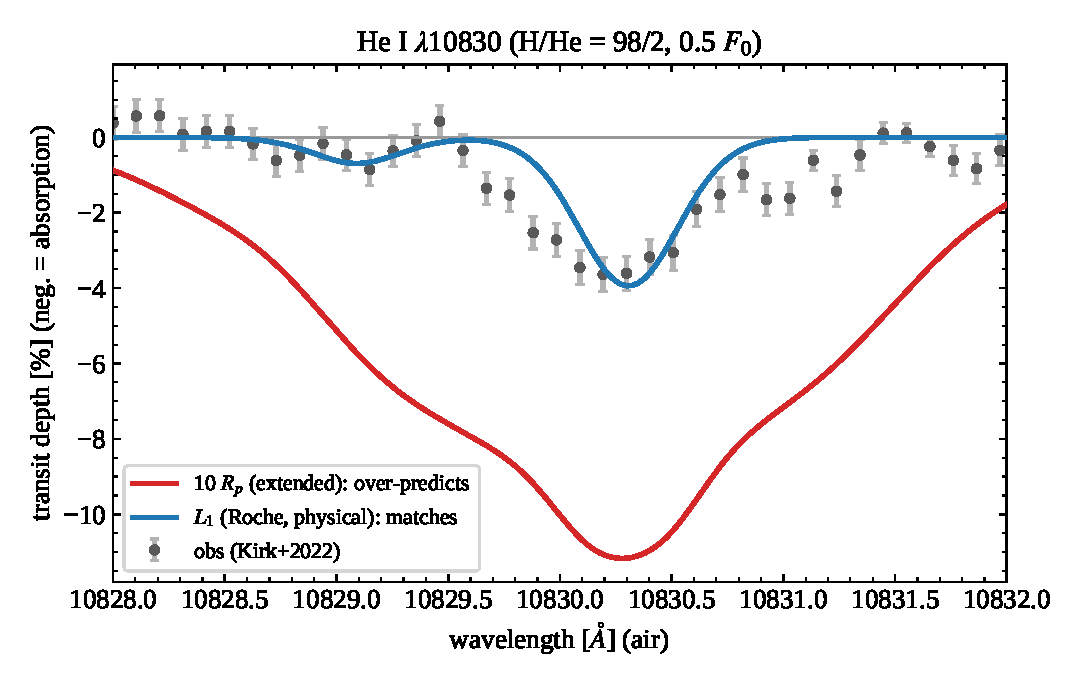
\includegraphics[width=0.99\linewidth]{he_compare.pdf}
\end{column}
\begin{column}{0.5\linewidth}\centering
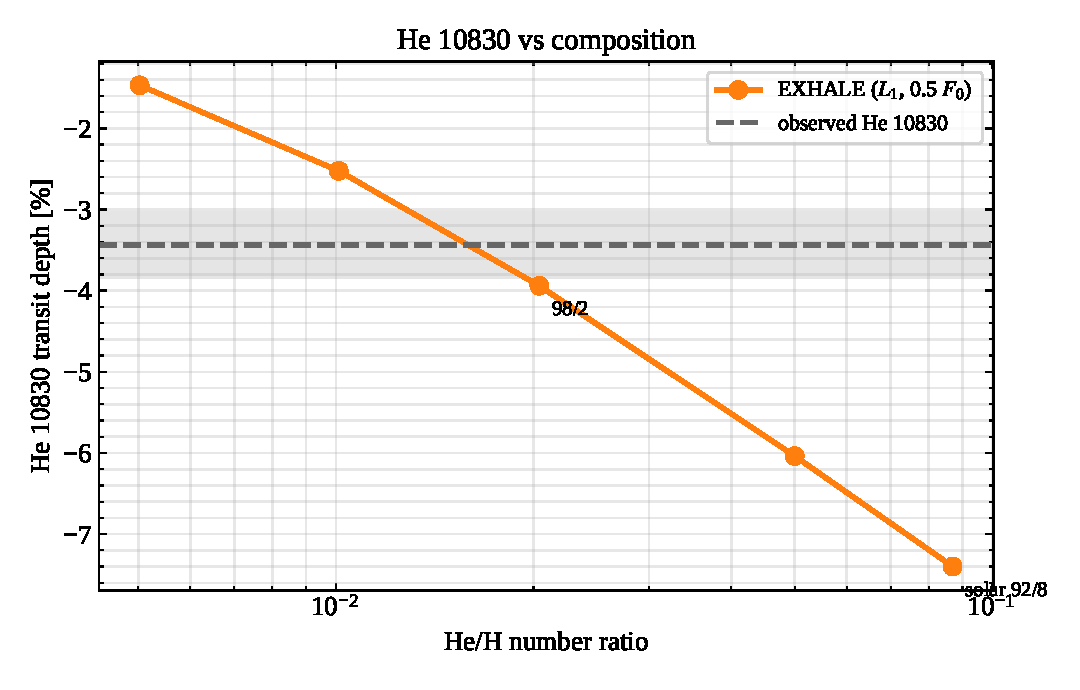
\includegraphics[width=0.99\linewidth]{hescan.pdf}
\end{column}
\end{columns}
\vspace{1mm}
\begin{itemize}
\item \textbf{Domain matters:} as in Yan+2022, extending to $10\,\Rp$ over-predicts
  the depth by $3$--$10\times$ ($72\%$ of the column from $r>L_1$, where 1-D spherical
  over-counts the $L_1$ funnel); the physical \textbf{$L_1$ (Roche)} domain matches.
\item \textbf{Composition:} solar (92/8) is too strong; matching the observed
  $\sim\!3.4\%$ requires a \textbf{He-depleted} atmosphere, $\mathbf{H/He\approx98/2}$
  ($\mathrm{He/H}\approx0.0204$).
\end{itemize}
\end{block}

\vfill

\begin{block}{6. H$\alpha$ via proper Ly$\alpha$ radiative transfer (LaRT)}
\begin{columns}[T]
\begin{column}{0.5\linewidth}\centering
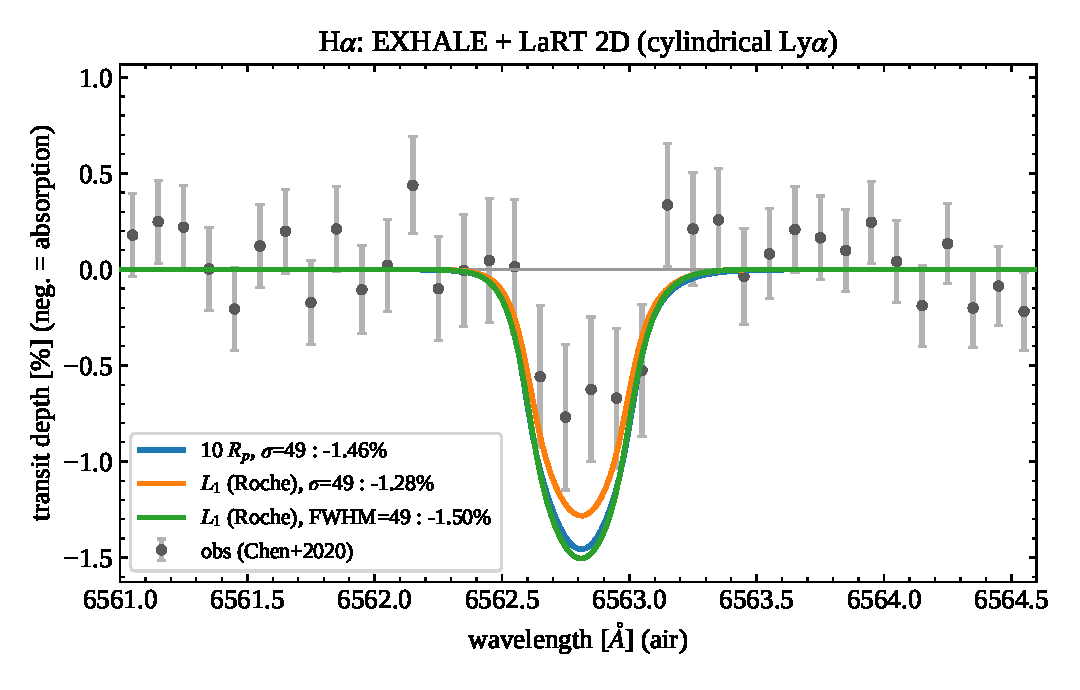
\includegraphics[width=0.99\linewidth]{halpha.pdf}
\end{column}
\begin{column}{0.5\linewidth}\centering
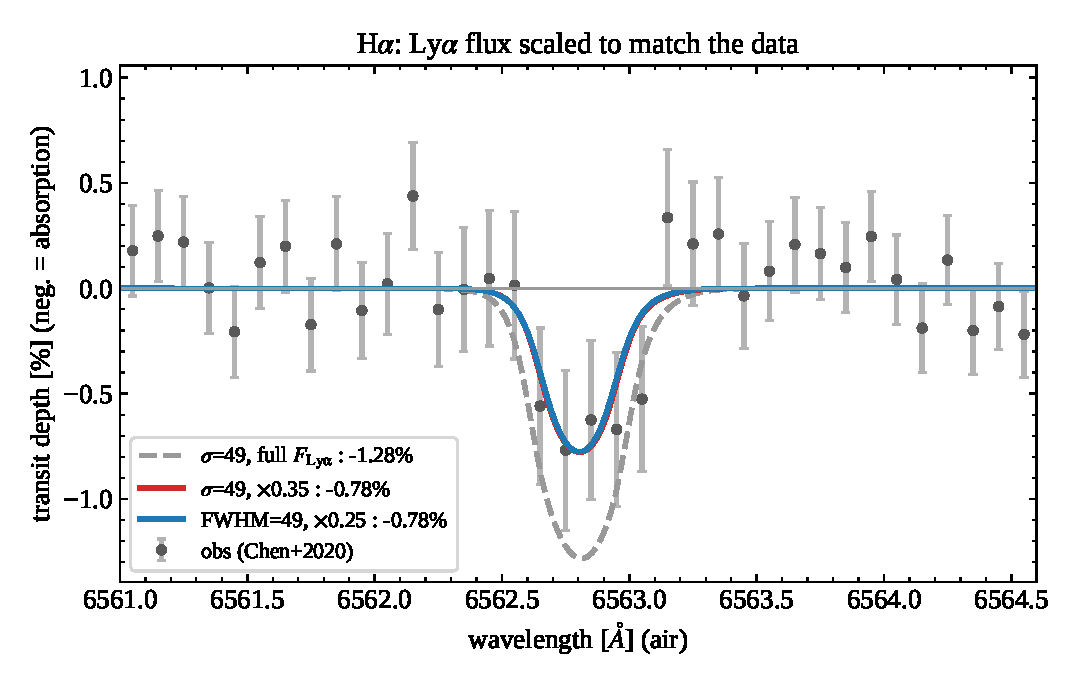
\includegraphics[width=0.99\linewidth]{halpha_matched.pdf}
\end{column}
\end{columns}
\vspace{1mm}
{\small
The \textbf{Ly$\alpha$ scattering (pump) rate} $P_\alpha$ [s$^{-1}$ atom$^{-1}$]
is built from the LaRT rate per unit luminosity $\mathcal{P}_{\rm LaRT}(\rho,z)$:
\[
P_\alpha \equiv B_{1s,2p}\,\bar J_\alpha
        = \mathcal{P}_{\rm LaRT}\,L_{\rm Ly\alpha}\,\frac{\Omega_\star}{4\pi},
\qquad
L_{\rm Ly\alpha}=\frac{F_{\rm Ly\alpha}\,4\pi a^2}{h\nu_\alpha}.
\]
The excited $n{=}2p$ population follows the Christie+2013 $2s/2p$ equilibrium,
\[
n_{2p}\simeq
\frac{(P_\alpha+C_{1s2p}n_e)\,n_{1s}+\alpha_{2p}n_e^2}
     {A_{2p1s}+(C_{2p1s}+C_{2p2s})n_e+\Gamma_{2p}}
\;\xrightarrow[\text{pump-dom.}]{}\;
n_{1s}\,\frac{P_\alpha}{A_{2p1s}},
\]
\par}
{\footnotesize ($\bar J_\alpha=P_\alpha/B_{1s,2p}$; $\Omega_\star/4\pi$ = stellar
solid-angle dilution; $\Gamma_{2p}$ = Balmer-continuum photoionization.)}
\vspace{1mm}
\begin{itemize}
\item Stellar illumination makes $P_\alpha$ (hence $n_{2p}$) \textbf{cylindrically
  symmetric} $\Rightarrow$ a 2-D $n_{2p}(\rho,z)$ integrator; incident Ly$\alpha$
  double-Gaussian ($\pm74$\,km/s, width 49\,km/s).
\item H$\alpha$ is \textbf{pump-dominated}, domain-\emph{insensitive}, depth
  $\propto F_{\rm Ly\alpha}$; matched at
  $\mathbf{F_{\rm Ly\alpha}\approx0.3\text{--}0.5\times}$ the $\epsilon$\,Eri proxy
  $\Rightarrow$ WASP-52's Ly$\alpha$ is $\sim\!1/3$--$1/4$ of the proxy.
\end{itemize}
\end{block}

\vfill

\begin{block}{7. Parameters that reproduce the observations}
\centering
\begin{tcolorbox}[colback=accent!10,colframe=accent,boxrule=1.2pt,sharp corners,
  left=4mm,right=4mm,top=3mm,bottom=3mm,width=\linewidth]
\renewcommand{\arraystretch}{1.15}
\begin{tabular}{@{}p{0.30\linewidth}p{0.63\linewidth}@{}}
\toprule
\textbf{Observable} & \textbf{Reproduced when} \\
\midrule
Mass loss $\Mdot$ & matches Yan+2022 within $\sim$10\% (\emph{no tuning}) \\
He\,10830 ($\sim\!3.4\%$) & $L_1$ (Roche) domain $+$ He-poor
  $\mathrm{H/He}\approx98/2$ ($\mathrm{He/H}\approx0.0204$) $+$ $0.5\,\Fo$ \\
H$\alpha$ ($\sim\!0.8\%$) & LaRT Ly$\alpha$ RT $+$
  $F_{\rm Ly\alpha}\approx0.3\text{--}0.5\times$ $\epsilon$\,Eri proxy \\
XUV hardness $\beta_m$ & $0.218$ \\
\bottomrule
\end{tabular}
\end{tcolorbox}
\end{block}

\vfill

\begin{block}{8. Conclusions}
\begin{itemize}
\item EXHALE$+$LaRT reproduce WASP-52b's He\,10830 \emph{and} H$\alpha$ with one
  self-consistent escape model; He\,10830 demands the \textbf{Roche ($L_1$) domain}
  and a \textbf{He-depleted} atmosphere ($\mathrm{H/He}\approx98/2$).
\item H$\alpha$, via proper Ly$\alpha$ RT, is a \textbf{diagnostic of the stellar
  Ly$\alpha$ flux} ($\approx1/3$--$1/4$ of the $\epsilon$\,Eri proxy). Jointly modeling the
  three lines breaks degeneracies among composition, $\Mdot$, and stellar Ly$\alpha$.
\item \textbf{Outlook:} we will extend this EXHALE$+$LaRT framework to a
  \textbf{systematic analysis of other exoplanet atmosphere observations}
  (He\,I\,10830 / H$\alpha$ / Ly$\alpha$), building a uniform grid of escape models.
\end{itemize}
\vspace{1mm}
{\scriptsize\textbf{Observations:} He\,I\,10830: Kirk et al.\ 2022 (AJ 164, 24;
Keck/NIRSPEC); H$\alpha$: Chen et al.\ 2020 (A\&A 635, A171; ESPRESSO/VLT).\\
\textbf{Model/theory:} Yan, Seon, Guo, Chen \& Li 2022 (ApJ 936, 177);
Caldiroli+2021 (A\&A 655, A30); Yang \& Guo 2018 (RAA 18, 077); Christie+2013
(ApJ 772, 144); Huang+2017 (ApJ 851, 150); Seon \& Kim 2020 (ApJS 250, 9).}
%% Model vintage: every number and figure above comes from the WASP-52b/fxuv*
%% case directories as they stood on 2026-08-09.  They predate the 2026-08-11
%% metal-line trapping / coronal-cutoff cooling and the corrected JFNK line
%% search and have NOT been re-converged under them.  The current production run
%% of this planet (10 R_p domain, full F_0, He/H = 0.0204) gives
%% log10 Mdot = 11.61 with ||R|| = 1.6e-4; that is a different configuration
%% from the L_1-domain, He-depleted best fit shown here, and is not this number.
%% STALE, second reason (P48; Update_EXHALE_stage1 section 137): every depth and every
%% spectrum above was computed with the profile files' GHOST rows included: the
%% two boundary rows at each end of every Hydro_ioniz/Ion_species file, which the
%% Python readers now drop. Measured shift on three states: 0.2--3.8 per cent on
%% the line-center and 4 A band depths. Values left exactly as measured;
%% regeneration awaits instruction.
%% The column body is exactly full: adding even one visible line to either
%% column overflows it (measured, 2026-08-11).
\end{block}

\end{minipage}
\end{column}
\end{columns}
\end{frame}
\end{document}
